\documentclass[9pt]{pnas-new}
% Use the lineno option to display guide line numbers if required.
% Note that the use of elements such as single-column equations
% may affect the guide line number alignment. 

\RequirePackage[english,slovene]{babel} % when writing in slovene
%\RequirePackage[slovene,english]{babel} % when writing in english

\templatetype{pnasresearcharticle} % Choose template 
% {pnasresearcharticle} = Template for a two-column research article
% {pnasmathematics} = Template for a one-column mathematics article
% {pnasinvited} = Template for a PNAS invited submission

\selectlanguage{slovene}
\etal{in sod.} % comment out when writing in english
\renewcommand{\Authands}{ in } % comment out when writing in english
\renewcommand{\Authand}{ in } % comment out when writing in english

\newcommand{\set}[1]{\ensuremath{\mathbf{#1}}}
\renewcommand{\vec}[1]{\ensuremath{\mathbf{#1}}}
\newcommand{\uvec}[1]{\ensuremath{\hat{\vec{#1}}}}
\newcommand{\const}[1]{{\ensuremath{\kappa_\mathrm{#1}}}} 

\newcommand{\num}[1]{#1}

\graphicspath{{./fig/}}

\title{Modeliranje evakuacije ljudi pred napadalcem z uporabo mehke logike}

% Use letters for affiliations, numbers to show equal authorship (if applicable) and to indicate the corresponding author
\author{Martin Božič}
\author{Marija Marolt}
\author{Jakob Maležič}

\affil{Poročilo seminarske naloge pri predmetu Skupinsko vedenje} 

\affil{Github projekta: https://github.com/Blarc/crowd-evacuation} 

% Please give the surname of the lead author for the running footer

\leadauthor{Maležič} % HEHE

\selectlanguage{english}

% Please add here a significance statement to explain the relevance of your work
\significancestatement{Crowd evacuation with assailants using fuzzy logic}{Each year a lot of terrorist attacks happen all over the world where a lot of people are killed or heavily damaged. With hope to decrease the casualties of such attacks, we present a crowd evacuation simulation that uses fuzzy logic to simulate the movement of people and assailants in different rooms. First we prepare models for achieving specific goals: obstacle avoidance, path searching and goal seeking. We then integrate these models together by setting a weight for each of the models, which determines how much each of the models affects the object's movement. We test the algorithm by simulating evacuation in different rooms that we prepared in advance. For better understanding of the simulation and creation of different rooms, user interface is implemented. The article and implementation is based on existing article \cite{Zhou2016}.}{Collective behaviour | Crowd evacuation | Fuzzy logic}

\selectlanguage{slovene}

% Please include corresponding author, author contribution and author declaration information
%\authorcontributions{Please provide details of author contributions here.}
%\authordeclaration{Please declare any conflict of interest here.}
%\equalauthors{\textsuperscript{1}A.O.(Author One) and A.T. (Author Two) contributed equally to this work (remove if not applicable).}
%\correspondingauthor{\textsuperscript{2}To whom correspondence should be addressed. E-mail: author.two\@email.com}

% Keywords are not mandatory, but authors are strongly encouraged to provide them. If provided, please include two to five keywords, separated by the pipe symbol, e.g:
\keywords{Skupinsko vedenje | Evakuacija ljudi | Mehka logika } 

\begin{abstract}
%To sem na hitro nekaj nakracal
Vsako leto se po celem svetu zgodi veliko napadov, kjer je ustreljenih in poškodovanih veliko ljudi. V tem članku, s pomočjo mehke logike, zgradimo različne modele, s katerimi lahko simuliramo takšne napade. Najprej predstavimo manjše modele, ki želijo doseči specifičen cilj - izogibanje oviram, iskanje poti in doseganje točke v prostoru. Te modele nato združimo v celoto tako, da jih ustrezno utežimo. Model testiramo in simuliramo v različnih prostorih z različnimi parametri. Za boljše razumevanje simulacije pripravimo tudi uporabniški vmesnik, ki simuliran napad vizualno prikaže. Naš model primerjamo še z ostalimi obstoječimi modeli.
\end{abstract}

\dates{\textbf{\today}}
\program{BM-RI}
\vol{2020/21}
\no{CB:GB} % group ID
%\fraca{FRIteza/201516.130}

\begin{document}

% Optional adjustment to line up main text (after abstract) of first page with line numbers, when using both lineno and twocolumn options.
% You should only change this length when you've finalised the article contents.
\verticaladjustment{-2pt}

\maketitle
\thispagestyle{firststyle}
\ifthenelse{\boolean{shortarticle}}{\ifthenelse{\boolean{singlecolumn}}{\abscontentformatted}{\abscontent}}{}

% If your first paragraph (i.e. with the \dropcap) contains a list environment (quote, quotation, theorem, definition, enumerate, itemize...), the line after the list may have some extra indentation. If this is the case, add \parshape=0 to the end of the list environment.
\dropcap{Z}biranje velikih gruč ljudi na javnih mestih je postalo nekaj neizogibnega. Na avtobusnih postajah, na železniški postaji, v velikih trgovskih centrih ali pa na koncertih in tekmah. Slednje lahko predstavlja veliko nevarnost za ljudi, kot tudi velik izziv za organizatorje in nadzornike takšnih javnih prostorov. Posebno pozornost je vredno nameniti predvidevanju potencialnih kriznih situacij, pri katerih je treba upoštevati nerazumno vedenje množice, ki nastopi kot posledica tesnobe in panike. V tem obziru je ključnega pomena razumevanje in razlikovanje značilnosti vedenja ljudi v običajnih ter kriznih situacijah.

Pri analizi dosedanjih napadov na množice, kot so streljanje v šolah~\cite{shootingWiki} in teroristični napadi na železniške postaje~\cite{CunmingWiki}, je prišlo do nekaj pomembnih spoznanj. Iracionalno evakuacijsko vedenje, slaba presoja varnosti stanovalcev ter malomarnost in nerazumne arhitekturne odločitve so vidno povečali škodo povzročenih napadov.

Preučevanje evakuacije množice lahko temelji na realnih poskusih ali računalniški simulaciji. Izvedeni so bili poskusi evakuacije pri zastoju na hodniku~\cite{bottlenecks2005}, v učilnici~\cite{classroom2008} ter nebotičniku~\cite{building2012}, ki so razkrili nekaj tipičnih vedenjskih vzorcev pri evakuaciji, kot so na primer tvorjenje vrst po principu zadrge~\cite{bottlenecks2005}, prilaščanje izhoda in čas priprave na evakuacijo~\cite{classroom2008}. V zadnjih nekaj desetletjih se vse bolj uporablja različne simulacijske modele. Helbing~\cite{Helbing2000} je predstavil model, ki simulira obnašanje ljudi v paniki pri evakuaciji. Pojasnil je zakaj pride do zastojev in poiskal optimalno rešitev. Varas~\cite{Varas2007} je uporabil model za odločanje s celičnim avtomatom za evakuacije sobe z ovirami. Upošteval je nerazumno vedenje v primeru panike in ob srečanju z oviro dodal faktor naključnosti reakcije v naslednjem koraku. Liu~\cite{Liu2009} je kasneje model nekoliko prilagodil. Obravnaval je tudi gostoto ljudi okoli izhoda. Poleg omenjenih so bili za preučevanje tega področja uporabljeni tudi drugi modeli. Izkazalo se je, da so rezultati močno odvisni od situacije in okolja.



\section*{Metode}
Za simulacijo evakuacije ljudi smo morali najprej pripraviti model za vodenje posameznega človeka. Posebej je bilo potrebno definirati vedenje napadalca.

V različnih študijah so pokazali, da je vid glavni vir informacij, na podlagi katerih, se človek v kriznih situacijah odloča o svojih dejanjih \cite{brcdp2018, mht2011}. Zato smo tudi mi zgradili modele, ki se odločajo na podlagi informacij iz okolice, vidne človeku. Vidno polje človeka je dodatno razdeljeno na sektorje in prikazano na sliki (\ref{fig:vision_field}). 

Naša implementacija temelji na modelu pešca in napadalca kot ju je definiral Zhou~\cite{Zhou2016}. Interes pešca je evakuacija in preživetje, na kar najbolj vplivajo lokacija cilja, napadalec in ovire. Na drugi strani je želja napadalca napasti čim več ljudi.

\begin{figure}
	\centering
	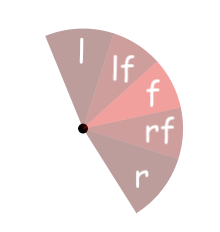
\includegraphics[scale=1.0]{fig/vidno_polje_osebe_2.png}
	\caption{Vidno polje osebe, razdeljeno na sektorje}
	\label{fig:vision_field}
\end{figure}

\subsection*{Mehka logika}
\label{mehka_logika}
Informacija, ki jo ljudje pridobimo iz okolice je odvisna od našega zaznavanja sveta in v večini primerih ni odvisna od meritev. Kako pridobljena informacija vpliva na posameznika pa je težko določiti s količino, saj se zmožnost zaznavanja razlikuje med posamezniki. Zato je smiselno, da informacije iz okolice opišemo z besedami in ne izmerljivimi količinami. Za opis lahko uporabimo množico mehkih pravil, ki jo je predstavil Zadeh \cite{ZADEH1965338} in se uporablja na različnih področjih. Največ v odločilnih sistemih \cite{Dong2013}, pri ocenjevanju zmogljivosti \cite{HWWDGHJZN1969}, napovedovalnih kontrolnih sistemih \cite{en10060794} ipd. Vpeljava pravil mehke logike je tudi veliko bolj robustna pri delu z netočnimi in negotovimi informacij, ki se jih pri sistemih, ki so odvisni od zaznavanja okolice, ne moremo izogniti.

\subsection*{Kategorije ljudi}
\label{kategorije_ljudi}
V osnovi ljudi razdelimo v tri kategorije. V tretjo kategorijo uvrščamo vse ljudi, kateri se v trenutni situaciji ne zavedajo prisotnosti napadalca. Takoj, ko se ti ljudje zavedajo napadalca, a ga v svojem vidnem polju ne vidijo, preidejo v drugo kategorijo. V prvo kategorijo posledično uvrščamo vse ljudi, ki napadalca vidijo, ali pa so ga videli v bližnji preteklosti in so s tem v napadalčevi neposredni nevarnosti. Ko človek enkrat preide v prvo ali drugo kategorijo, v trenutni simulaciji ne more več preiti v tretjo kategorijo ljudi, saj se zavedanja o napadalcu ne more znebiti.

\subsection*{Lokalno izogibanje oviram}
\label{lokalno_izogibanje_oviram}
Metoda lokalnega izogibanja oviram poskrbi, da se osebe izognejo oviram, ki se nahajajo pred njimi in so dovolj blizu, da jih oseba zazna. Metoda deluje na podlagi vnaprej določenih pravil mehke logike. Vhode predstavljajo najbližje ovire v posameznih sektorjih vidnega polja, izhoda pa sta smer ($\alpha$) in hitrost gibanja ($V$). Vhodi so predstavljeni z mehko množico \{BLIZU, DALEČ\}, izhoda pa sta predstavljena z mehkima množicama \{Močno-Poz, Malo-Poz, Nič, Malo-Neg, Močno-Neg\} in \{USTAVITEV, POČASI, HITRO\}. Pravila mehke logike metode lokalnega izogibanja oviram lahko sedaj povzamemo z:
\begin{equation}
\label{lokalno_izogibanje_oviram_summarize}
\begin{bmatrix}
\delta_{\alpha}\\
\delta_{V}
\end{bmatrix} = R_{0} (d_{o}^{l}, d_{o}^{fl}, d_{o}^{f}, d_{o}^{fr}, d_{o}^{r})
\end{equation}

\noindent Z opisanimi mehkimi množicami dobimo 32 (oziroma $2^5$) pravil ($R_0$), ki so opisana v tabeli \ref{rules_obstacle_avoidance_behaviour}.

\begin{table}[]
\centering
\begin{tabular}{|l|lllll|ll|}
\hline
\textbf{Zap. št.} & \multicolumn{5}{l|}{\textbf{Vhod}} & \multicolumn{2}{l|}{\textbf{Izhod}} \\ 
\cline{2-8} 
\textbf{pravila} & ${d_l}$ & ${d_{fl}}$ & ${d_{fl}}$ & ${d_{fl}}$ & ${d_{fl}}$ & ${\alpha}$ & V \\ 
\hline
1   & BLIZU & BLIZU & BLIZU & BLIZU & BLIZU & Nič           & USTAVITEV  \\ \hline
2   & BLIZU & BLIZU & BLIZU & BLIZU & DALEČ & Močno-Poz     & POČASI     \\ \hline
3   & BLIZU & BLIZU & BLIZU & DALEČ & BLIZU & Malo-Poz      & POČASI     \\ \hline
4   & BLIZU & BLIZU & BLIZU & DALEČ & BLIZU & Močno-Poz     & POČASI     \\ \hline
5   & BLIZU & BLIZU & BLIZU & DALEČ & BLIZU & Nič           & HITRO      \\ \hline
\dots & \dots  & \dots  & \dots  & \dots  & \dots  & \dots  & \dots      \\ \hline
31  & DALEČ & DALEČ & DALEČ & DALEČ & BLIZU & Nič           & HITRO      \\ \hline
32  & DALEČ & DALEČ & DALEČ & DALEČ & DALEČ & Nič           & HITRO      \\ \hline
\end{tabular}
\caption{Sistem pravil mehke logike $R_0$ pri metodi lokalnega izogibanja oviram.}
\label{rules_obstacle_avoidance_behaviour}
\end{table}

\subsection*{Iskanje poti}
\label{iskanje_poti}
Pri metodi iskanja poti na spremembo trenutne hitrosti in smeri posamezne osebe najbolj vplivajo hitrosti in smeri ostalih oseb v vidnem spektru osebe. Tako bi pri metodi iskanja poti na trenutno osebo najbolj vplivala oseba, ki se proti izbrani osebi premika z veliko hitrostjo v nasprotni smeri. Metoda vedno vodi posameznika po najvarnejši poti, tako da se vedno izogiba področjem z visoko negativno energijo. Moč negativne energije se izračunava sproti in je odvisna od trenutnega vpliva ovir in trenutne nevarnosti trčenja posameznika z ostalimi osebami. Kot vpliv ovire v večini upoštevamo zidove, pohištvo in ostale stacionarne reči v vidnem sektorju posameznika. Vpliv ovir označimo z oznako ${(OI^*)}$, pri čemer sistem mehke logike za izračun trenutnega vpliva ovir opišemo z enačbo (\ref{OI_equation}).

\begin{equation}
\label{OI_equation}
OI_{i}^* = R_{1}(\phi^*_{oi}, d^*_{oi})
\end{equation}

\noindent ${\phi^*_{oi}}$ predstavlja v katerem kotu vidnega spektra posameznika se ovira nahaja, ${d^*_{oi}}$ predstavlja razdaljo od posameznika do posamezne ovire in ${R_{1}}$ predstavlja zbirko pravil mehke logike. Pri njej velja, da imajo večji vpliv na rezultat bližnje ovire z večjim kotom zaviranja pogleda osebe.


Nevarnost trčenja opazovane osebe z drugo osebo v prostoru označimo z oznako ${(CR^*)}$, pri čemer sistem mehke logike opišemo z enačbo (\ref{CR_equation}).

\begin{equation}
\label{CR_equation}
CR_{j}^* = R_{2}(d^*_{oi}, V_{j}^*, \theta_{pj}^*)
\end{equation}

\noindent ${V_{j}^*}$ predstavlja trenutno hitrost neke druge osebe, ${\theta_{pj}^*}$ predstavlja kot med smerjo gibanja te osebe glede na trenutno opazovano osebo in ${d^*_{pj}}$ predstavlja razdaljo od druge osebe do trenutno opazovane osebe. ${R_{2}}$ predstavlja zbirko pravil mehke logike, pri kateri je glavno vodilo, da je tveganje trka nizko, če oseba stoji pri miru ali je ovira daleč oziroma dovolj oddaljena od smeri gibanja. Celotno negativno energijo trenutne opazovane osebe izračunamo z enačbo (\ref{NE_equation}),

\begin{equation}
\label{NE_equation}
NE^* = k_{w} \cdot OI^* + (1 - k_{w}) \cdot CR^*,
\end{equation}

\noindent kjer ${OI^*}$ predstavlja vsoto vseh ${OI_{i}^*}$, za vsak predmet v vidnem spektru osebe in ${CR^*}$ predstavlja vsoto vseh izračunanih nevarnosti trčenja ${CR_{j}^*}$, za vsako drugo osebo, ki se giblje v vidnem prostoru trenutne osebe. ${k_{w}}$ predstavlja faktor uteži, s katerim lahko nadziramo pomembnost vrednosti OI in CR.


\subsection*{Doseganja cilja}
\label{doseganje_cilja}
Pri metodi doseganja cilja, se opazovana oseba vedno nagiba k temu, da se pomika proti končnemu cilju. Opišemo jo z ${d_g}$, ki predstavlja razdaljo do cilja in ${\gamma_{g}}$, ki predstavlja kot, glede na orientacijo trenutne osebe in smerjo cilja. Razdaljo ${d_g}$ opišemo z dvema \{BLIZU, DALEČ\}, kot ${\gamma_{g}}$ pa s petimi \{Močno-Neg, Malo-Neg, Nič, Malo-Poz, Močno-Poz\} stanji mehke logike. Sistem pravil mehke logike pri metodi doseganja cilja je predstavljen v tabeli (\ref{rules_goal_seeking_behaviour}). Pri čemer ${\alpha}$ predstavlja končni kot, $V$ pa predstavlja hitrost premika opazovane osebe.

% \usepackage{multirow}
\begin{table}[]
\centering
\begin{tabular}{|l|ll|ll|}
\hline
\textbf{Zap. št.} & \multicolumn{2}{l|}{\textbf{Vhod}} & \multicolumn{2}{l|}{\textbf{Izhod}} \\ \cline{2-5} 
\textbf{pravila} & ${\gamma_{g}}$          & ${d_g}$          & ${\alpha}$           & $V$         \\ \hline
1                            & Močno-Poz  & BLIZU & Močno-Neg  & USTAVITEV  \\ \hline
2                            & Močno-Poz & DALEČ & Močno-Neg   &  POČASI           \\ \hline
3                            & Malo-Poz &  BLIZU &   Malo-Neg   &  POČASI   \\ \hline
4                            & Malo-Poz & DALEČ &  Malo-Neg  &  POČASI   \\ \hline
5                            & Nič      &  BLIZU &  Nič    &   HITRO    \\ \hline
6                            & Nič      & DALEČ  &  Nič    &   HITRO  \\ \hline
7                            & Malo-Neg & BLIZU & Malo-Poz    &  POČASI   \\ \hline
8                            & Malo-Neg & DALEČ & Malo-Poz   &  POČASI    \\ \hline
9                            & Močno-Neg & BLIZU &  Močno-Poz   & USTAVITEV \\ \hline
10                           & Močno-Neg & DALEČ  &  Močno-Poz   &  POČASI   \\ \hline
\end{tabular}
\caption{Sistem pravil mehke logike $R_4$ pri metodi doseganja cilja.}
\label{rules_goal_seeking_behaviour}
\end{table}

\subsection*{Utežena vsota}
Končno hitrost $V$ in končni kot premika ${\alpha}$ trenutne osebe izračunamo z metodo utežene vsote rezultatov metode lokalnega izogibanja oviram \ref{lokalno_izogibanje_oviram}, metode iskanja poti \ref{iskanje_poti} in metode doseganja cilja\ref{doseganje_cilja}. Pomembnost rezultata vsake metode utežimo s faktorji ${\delta_{ao}}$, ${\delta_{ap}}$ in ${\delta_{ag}}$, ki določajo pomembnost posamezne metode. Vsak faktor opišemo s tremi stanji mehke logike, \{MANJŠI, SREDNJI, VELIK\}. Vrednosti faktorjev določamo sproti po enačbi (\ref{delta_equation}),



\begin{equation}
\label{delta_equation}
\begin{bmatrix}
\delta_{ao}\\
\delta_{ap}\\
\delta_{ag}
\end{bmatrix} = R_{5} (d_{o}^f, \overline{NE^f}, d_{g})
\end{equation}

\noindent pri čemer ${d_{o}^f}$ predstavlja razdalijo do ovire, ki stoji pred opazovano osebo, ${\overline{NE^f}}$ predstavlja velikost negativne energije, v prostoru pred opazovano osebo, in ${d_{g}}$ predstavlja razdaljo od trenutno opazovane osebe do cilja. ${R_{5}}$ predstavlja nabor pravil mehke logike. 

\subsection*{Uporabniški vmesnik}
Uporabniški vmesnik smo naredili z uporabo knjižnice p5.js. Slednja temelji na jeziku Processing in prikazuje potek simulacije. Kot je prikazano na sliki (\ref{uporabniski_vmesnik_fig}) lahko uporabnik na enostaven način kreira in požene simulacijo.

Prostor spreminja z vnosom želene dimenzije v slikovnih pikah. Vanj vrisuje ovire in dodatnw zidove iz kvadratkov. Tem nastavi velikost od 1 do 10, pri čemer 1 predstavlja kvadrat s stranicami dolžine 20 slikovnih pik na zaslonu. Ima tudi možnost izbrisa posameznih blokov. 

V prostor postavi ljudi, ki sledijo globalnem cilju ali imajo svoj cilj. Pozicijo globalnega cilja je možno spremeniti. Med samo simulacijo lahko prekinemo sledenje ljudi globalnemu cilju oziroma ga nato nazaj vzpostavimo. Poleg tega imamo možnost prikaz vidnega polja vklopiti ali izklopiti. Posebej postavimo napadalca in prikažemo njegov vidni kot.

Svoje nastavitve simulacije je možno izbrisati ali shraniti na svoj računalnik v obliki datoteke json. Prav tako imamo preko uporabniškega vmesnika možnost uporabiti vnaprej pripravljene prostore, zapisane v datoteko json.

Med simulacijo prikazujemo število preživelih, mrtvih, pešcev, napadalcev ter čas trajanja in število sličic na sekundo. Simulacijo lahko začasno ustavimo in nato zopet nadaljujemo z njenim izvajanjem.

\begin{figure}
	\centering
	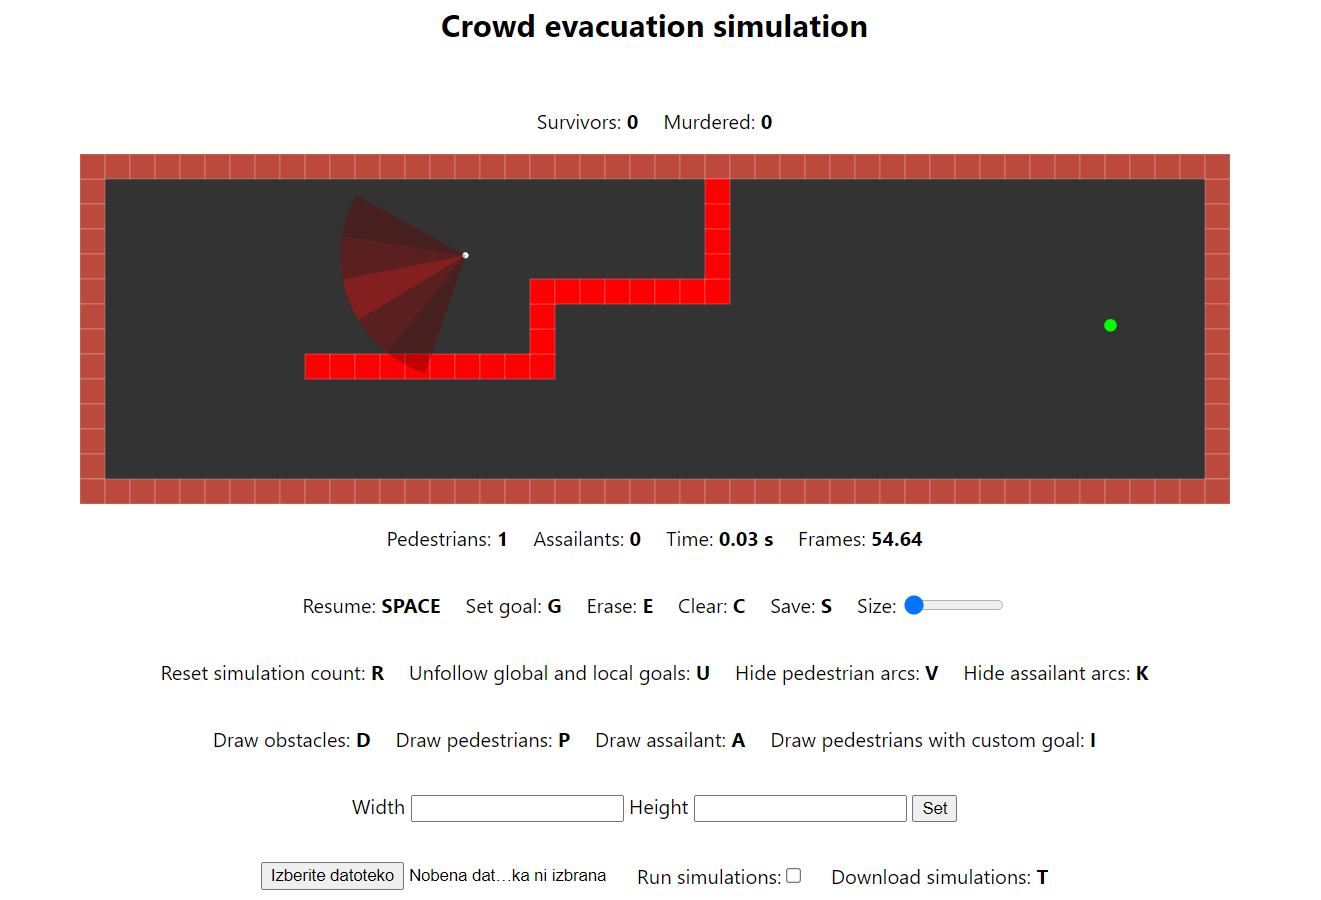
\includegraphics[scale=0.4]{fig/uporabniski_vmesnik_razsirjen.png}
	\caption{Primer uporabniškega vmesnika z legendo.}
	\label{uporabniski_vmesnik_fig}
\end{figure}


% TODO (uporabniski vmesnik): opis uporabniskega vmesnika do sedaj (risanje zidov, postavljanje globalnega in lokalnih ciljev)
% slika uporabniskega vmesnika
% popravi sliko osebe, obrez brez zelenega ozadja

%todo (rezultati): pripravimo razlicne prostore, podamo slike prostorov in opisemo kaj bomo merili (koliko jih prezivi, koliko casa rabijo do uspesne evakuacije) - poglej clanek kaj so se tam merili

\section*{Rezultati}
Velikega pomena je izvajanje simulacije v realnem času. Gibanje ljudi je hitro, zato je tudi samo z opazovanjem možno videti določena tipična vedenja in vzorce pri evakuaciji. Ker je simulacija javno objavljena in prosto dostopna, služi kot učni in testni pripomoček ostalim raziskovalcem na tem področju.

Generirali smo simulacije v sobah enake dimenzije z različnim številom ljudi in različnim številom izhodov. Pri tem smo merili kako se spreminja število preživelih in mrtvih s časom. Med sabo smo primerjali hodnike na katerih je bilo različno število ljudi in sobe, ki so se razlikovale v številu izhodov. Primer hodnika je prikazan na sliki (\ref{primer_hodnika_fig}). Primer sobe z enim izhodom pa vidimo na sliki (\ref{primer_sobe_fig}).

\begin{figure}
	\centering
	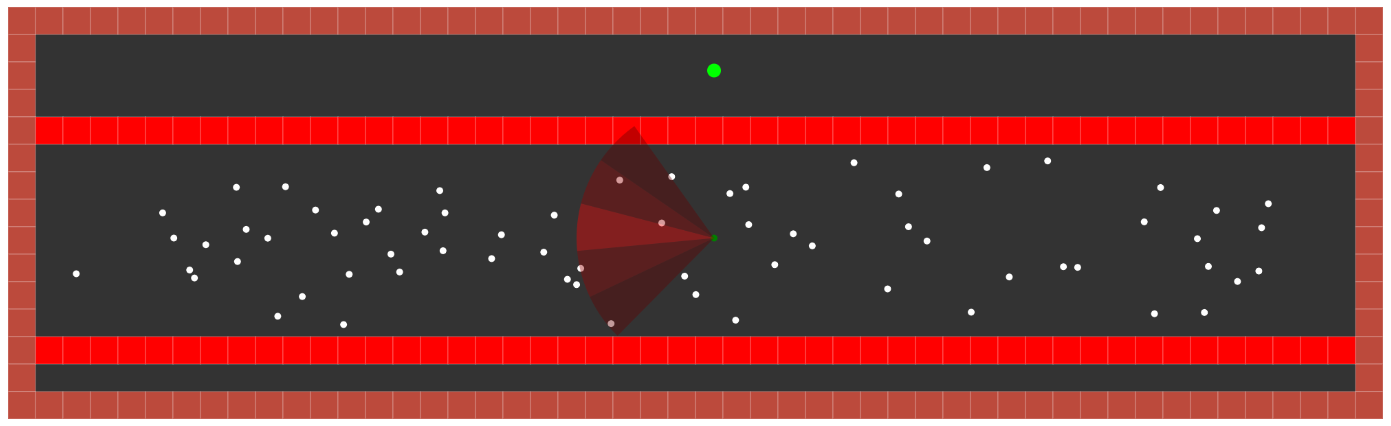
\includegraphics[scale=0.333]{fig/hallway.png}
	\caption{Primer evakuacije ljudi na hodniku z napadalcem}
	\label{primer_hodnika_fig}
\end{figure}

\begin{figure}
	\centering
	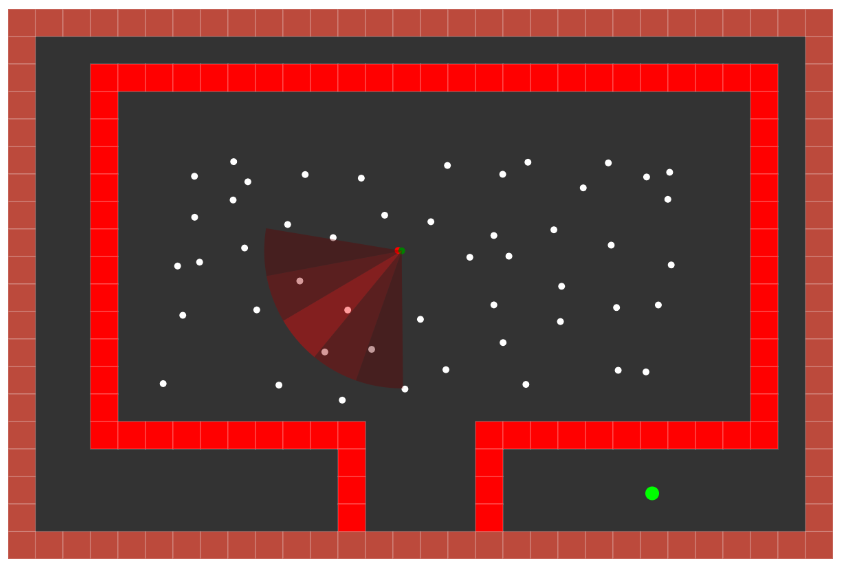
\includegraphics[scale=0.3]{fig/room_with_one_exit.png}
	\caption{Primer evakuacije ljudi v prostoru z napadalcem in enim izhodom}
	\label{primer_sobe_fig}
\end{figure}

Če primerjamo rezultate simulacij na hodniku, predstavljenih na sliki (\ref{primer_hodnika_fig}), vidimo, da nekoliko manjši procent ljudi preživi pri večjem številu ljudi. To lahko pripišemo veliki gneči, ki
nastane pri izhodu. Ljudje v tej gneči so namreč lažja tarča za napadalca.

\begin{figure}
	\centering
	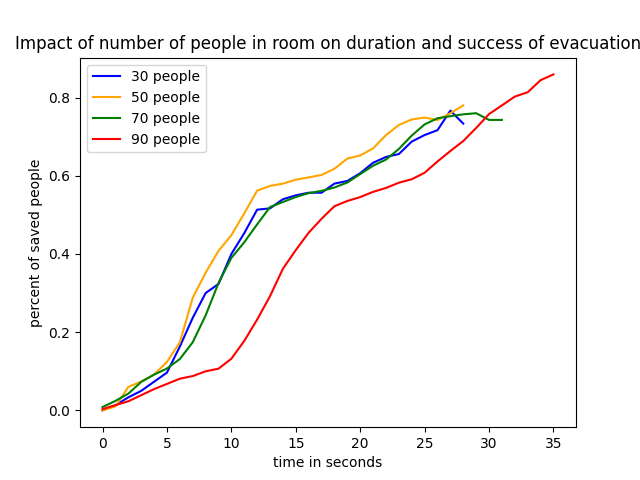
\includegraphics[scale=0.5]{fig/hallway_evacuation_procent.png}
	\caption{Vpliv števila ljudi na trajanje in uspešnost evakuacije}
	\label{hodnik_fig}
\end{figure}

Pri primerjavi simulacij v sobah z različnim številom izhodov smo dobili rezultate, ki so prikazani na sliki (\ref{soba_fig}). Opazno je, da je procent preživelih pri sobah z večjim številom izhodov večji. Ljudje imajo v teh primerih več možnosti za pobeg. Pred posameznim izhodom, kjer je nevarnost napada največja, nastane manjši zastoj in posledično imamo manjši procent žrtev.

\begin{figure}
	\centering
	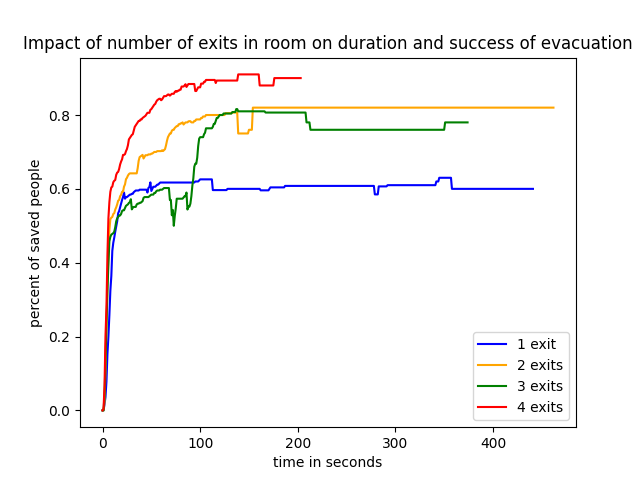
\includegraphics[scale=0.5]{fig/room_evacuation_procent.png}
	\caption{Vpliv števila ljudi na trajanje in uspešnost evakuacije}
	\label{soba_fig}
\end{figure}


V naših poskusih ljudje nimajo predhodnega znanja, npr. o prostoru ali napadalcu, kar v realni situaciji ni vedno res. Ljudje bi se med sabo lahko obvestili, da so v nevarnosti. V realnem življenju bi začeli npr. kričati in opozarjati druge.

Druga pomanjkljivost naše simulacije je naključno premikanje napadalca. Bolje bi bilo, da bi se napadalec potepal naokoli, ne pa premikal naključno. Najbolj je to opazno, ko je prostor okoli njega prazen. Takrat bi v realni situaciji naredil obhod prostora, pri naključnem premikanju pa se dlje časa zadržuje v bližnji okolici.


\section*{Sklep}
V članku smo obravnavali različne modele mehke logike z različnim številom peščev, napadalcev in različnimi okoliščinami. 
Posebej smo obravnavali metode lokalnega izogibanja oviram, iskanja poti ter doseganja cilja. Končni rezultat je predstavljen kot njihova utežena vsota. 
Velika prednost uporabe mehke logike je učinkovito opisovanje informacij iz okolice pri simulaciji, zaradi česar so nastale simulacije močno realistične.

Osredotočili smo se na izdelavo čim boljše simulacije za predstavitev različnih situacij v realnem času. Omogoča spreminjanje številnih ključnih parametrov, ki so zanimivi pri preučevanju evakuacije ljudi ter evakuacije ljudi v prostoru z napadalcem. 

Ugotovili smo, da obstaja povezava med številom ljudi v prostoru in časom evakuacije. Ta pri naših poskusih ni najbolj razvidna, a to pripisujemo majhni učni množici. Iz poskusov v sobah z različnim številom izhodov smo uspeli ugotoviti, da večje število izhodov poveča možnosti za preživetje.

Nadaljnje raziskave bi bile lahko usmerjene v dodatno izvedbo in analizo simulacij. Če bi izvedli večje število poskusov, bi bili rezultati morda drugačni oziroma natančnejši. V naših poskusih ljudje nimajo predhodnega znanja, npr. o prostoru ali napadalcu, kar v realni situaciji ni vedno res. Prav tako bi premikanje napadalca, ki je trenutno naključno, če ne vidi nobenega človeka, naključno. Zanimivo bi bilo tudi omogočiti ročno premikanje napadalca in oblikovanje simulacije kot računalniške igre.


\acknow{MB je implementiral metode in izvedel simulacije, MM je skrbela za poročilo in analizirala rezultate, JM je implementiral in optimiziral uporabniški vmesnik.}
\showacknow % Display the acknowledgments section

% \pnasbreak splits and balances the columns before the references.
% If you see unexpected formatting errors, try commenting out this line
% as it can run into problems with floats and footnotes on the final page.
%\pnasbreak

\begin{multicols}{2}
\section*{\bibname}
% Bibliography
\bibliography{./bib/bibliography}
\end{multicols}

\end{document}